\documentclass{beamer}

\usepackage{Vor2018glærur}

\title{Tölvunarfræði 2}
\subtitle{Vika 2}

\begin{document}

\begin{frame}
\titlepage
\end{frame}

\section{Breytur og minni í C++}

\begin{frame}{Líftími breyta}
    \begin{itemize}
        \item Við munum að breytur hafa mismunandi líftíma
        \begin{itemize}
            \item Aðskilið hugtak: gildissvið breytu \eng{variable scope}
        \end{itemize}
        \item Í C++ getur líftími breytu verið af nokkrum gerðum, þá helst
        \begin{itemize}
            \item Sjálfvirkur \eng{automatic} - líftími breytunnar er ákvarðaður sjálfkrafa
            \item Kvikstæður \eng{dynamic} - breytan lifir meðan forritari segir
            \item Kyrrstæður \eng{static} - breytan lifir meðan forritið keyrir
        \end{itemize}
        \item Í flestum forritunarmálum sem við erum líkleg til að hafa skoðað hingað til sér ruslasafnari \eng{garbage collector} um að hreinsa til, en venjulegt C++ hefur ekki slíkan
    \end{itemize}
\end{frame}

\begin{frame}{Minnissvæði í C++}
    \begin{itemize}
        \item Í keyrandi C++ forriti eru (venjulega) nokkrar gerðir minnis í gangi á hverjum tímapunkti
        \begin{itemize}
            \item Þula \eng{code segment}. Geymir upplýsingar um forritið - vélamálsskipanir og fasta, venjulega er eingöngu lesaðgangur
            \item Gagnasvæði \eng{data segment}.
            Frátekið í upphafi keyrslu, getum ekki stækkað eða minnkað.
            \item Hlaði \eng{stack}. Minnissvæði af breytilegri stærð sem hægt er að fá aðgang að á skipulegan máta
            \item Kös \eng{heap}. Er úthlutað og skilað að beiðni forritsins, minnisdreifing ekki endilega mjög fyrirsjáanleg
        \end{itemize}
        \item Hlaðinn og kösin eru þau svæði sem við þurfum að skoða sérstaklega
    \end{itemize}
\end{frame}

\begin{frame}{Hvað fer svo hvert?}
    \begin{itemize}
        \item Þumalputtareglur fyrir ``venjulegt'' C++
        \begin{itemize}
            \item Víðværar \eng{global} breytur fara í gagnasvæðið
            \item Líftími staðværra \eng{local} breyta er ákvarðaður sjálfkrafa og þær eru settar á hlaðann
            \item Kvikstæðar breytur fást með sérstökum minnisúthlutunaraðgerðum eins og \texttt{new} og eru settar í kös
        \end{itemize}
    \end{itemize}
\end{frame}

\begin{frame}{Hlaðinn}
    \begin{columns}
        \column{0.6\textwidth}
        \begin{itemize}
            \item Hlaðinn er ``lítið'' minnissvæði sem C++ forrit nota til að halda utan um staðværar breytur og upplýsingar um fallsköll
            \begin{itemize}
                \item Getum lent í því að hlaðinn fyllist
            \end{itemize}
            \item Uppbygging er skipuleg (LIFO)
            \begin{itemize}
                \item Hentar vel fyrir raunverulega örgjörva, gerir mjög hraða vinnslu mögulega
            \end{itemize}
            \item Líftíma breyta á hlaðanum er stjórnað sjálfkrafa í C++, minninu er skilað þegar viðkomandi fall lýkur keyrslu
        \end{itemize}
        \column{0.3\textwidth}
        \pause
        \begin{center}
            
\includegraphics[width=\linewidth]{stack-overflow}

            Logo \href{https://stackoverflow.com/}{stackoverflow.com}
        \end{center}
    \end{columns}
\end{frame}

\begin{frame}{Uppbygging hlaðans}
    \begin{columns}
        \column{0.5\textwidth}
        \begin{itemize}
            \item Uppbygging hlaðans þegar \texttt{DrawSquare} kallar á \texttt{DrawLine}
            \item Mynd: \href{https://en.wikipedia.org/wiki/File:Call\_stack\_layout.svg}{Wikimedia}
        \end{itemize}
        \column{0.5\textwidth}
        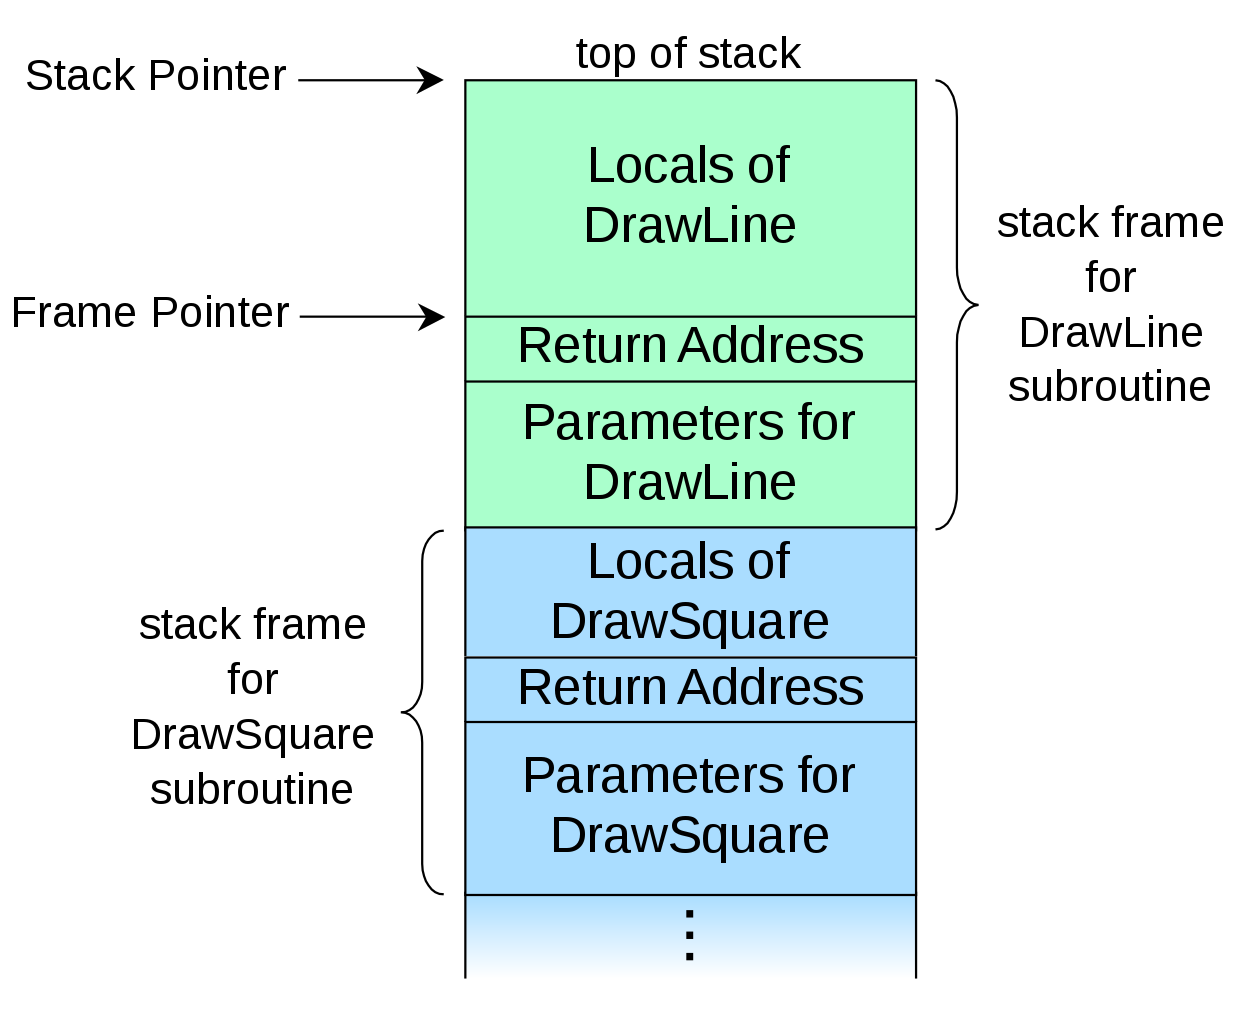
\includegraphics[width=\linewidth]{call-stack-layout}
    \end{columns}
\end{frame}

\begin{frame}{Kösin}
    \begin{itemize}
        \item Kösin er ``stórt'' minnissvæði sem C++ forrit geta beðið um skerf af á keyrslutíma
        \item Er ekki endilega samfellt, getur verið mjög uppskipt \eng{fragmented}
        \item Hægur aðgangur í samanburði við aðgang að hlaðanum
        \item Hægt er að fá aðgang að kösinni hvaðan sem er úr forritinu
        \begin{itemize}
            \item Takmarkast ekki við fallskall
        \end{itemize}
        \item C++ forrit sem tekur frá svæði í kös þarf að skila því aftur!
    \end{itemize}
\end{frame}

\subsection{Upprifjun á bendum}

\begin{frame}{Bendar}
    \begin{itemize}
        \item Bendir er breyta sem inniheldur staðsetningu minnissvæðis
        \begin{itemize}
            \item Hún ``bendir á'' minnissvæðið
        \end{itemize}
        \item Hægt er að nota bendinn til að fá aðgang að gögnunum sem geymd eru í minnissvæðinu
        \begin{itemize}
            \item {\color{red} Nýtt}: Gagnlegt þegar gögnin eru í kös!
        \end{itemize}
    \end{itemize}
    
    \begin{center}
    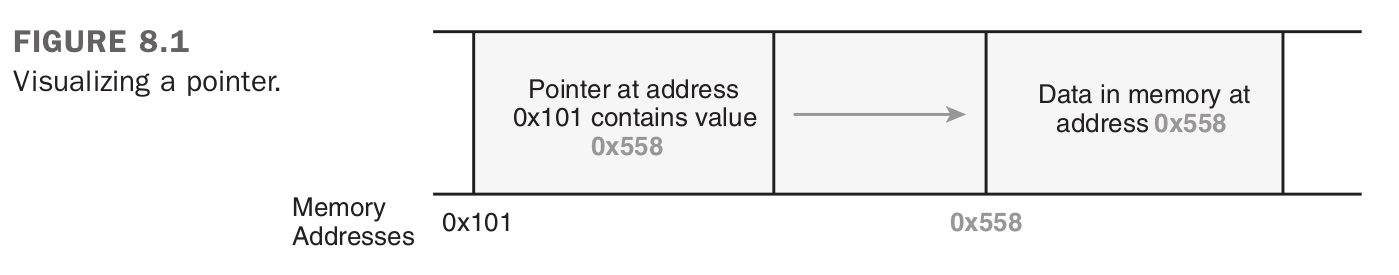
\includegraphics[width=\textwidth]{pointer-visualization}
    \end{center}
\end{frame}

\begin{frame}[fragile]{Bendar}
    Við getum búið til bendi sem vísar á breytu af gerðinni \texttt{gerd} með \texttt{gerd*}, náð í  staðsetningu minnissvæðis með \texttt{\&} virkjanum og sótt gögn sem bendir vísar á með \texttt{*} virkjanum

    \cppfile[firstline=6, lastline=15, gobble=4, fontsize=\small, label=dereferencing.cpp]{Code/w1/dereferencing.cpp}
\end{frame}

\begin{frame}[fragile]{Nýtt: New}
    Notum \texttt{new} til að taka frá minnissvæði í kös fyrir breytu og skila bendi á minnissvæðið.
    \begin{minted}[fontsize=\small, frame=lines]{cpp}
// request memory for one element
Type* pointer = new Type;
// request memory for numElements
Type* pointer = new Type[numElements];
    \end{minted}
    Til að taka frá minni í kös fyrir heiltölur:
    \begin{minted}[fontsize=\small, frame=lines]{cpp}
// get a pointer to an integer
int* pointToAnInt = new int;
// pointer to a block of 10 integers
int* pointToNums = new int[10];
    \end{minted}
\end{frame}

\begin{frame}[fragile]{new og delete}

    \cppfile[firstline=11, lastline=18, gobble=4, fontsize=\small, label=dynamicdouble.cpp]{Code/w2/dynamicdouble.cpp}

\end{frame}

\begin{frame}{Föll og breytur í C++}
    \begin{itemize}
        \item Við höfum töluverða stjórn á hvernig C++ meðhöndlar inntaksbreytur og skilabreytur
        \item Sjálfgefið er að C++ noti gildisviðföng \eng{value passing}
        \begin{itemize}
            \item En stundum er það ekki skilvirkt
            \item Stundum er það það ekki mögulegt
        \end{itemize}
        \item Annar möguleiki: Taka inn og skila bendum
    \end{itemize}
\end{frame}

\begin{frame}{Bendar sem inntaksbreytur}
    Skoðum \texttt{incrementpointervalue.cpp} og \texttt{pointerpassing.cpp}.
\end{frame}

\section{Fylki og listar}

\begin{frame}{Meira um fylki í C++}
    Munum: ``gamaldags'' fylki í C++ eru þunn skel utan um benda.

    \cppfile[firstline=7, lastline=9, gobble=4, label=arraysandpointers.cpp]{Code/w2/arraysandpointers.cpp}
    Þetta setur takmarkanir á hvernig hægt er að nota fylki sem inntaks- og úttaksbreytur.
\end{frame}

\begin{frame}{Fylki sem bendar}
    Tvær leiðir til að skrifa út stökin sem eru í þriggja staka fylkinu \texttt{pizzaSizes}
    \begin{columns}
        \column{0.45\textwidth}
        \cppfile[firstline=10, lastline=17, gobble=4, label=arraysandpointers.cpp, fontsize=\scriptsize, linenos=false]{Code/w2/arraysandpointers.cpp}
        \column{0.55\textwidth}
        \cppfile[firstline=22, lastline=27, gobble=4, label=arraysandpointers.cpp, fontsize=\scriptsize, linenos=false]{Code/w2/arraysandpointers.cpp}
    \end{columns}
\end{frame}

\begin{frame}{Takmarkanir fylkja}
    \begin{itemize}
        \item Fylki eru föst að stærð eftir að minni hefur verið úthlutað
        \begin{itemize}
            \item Til að breyta stærð fylkis þarf að úthluta nýju fylki og afrita gögnin
        \end{itemize}
        \item Önnur leið til að geyma runu af gögnum - listi
        \begin{itemize}
            \item Klassískur listi samanstendur af hnútum \eng{nodes} af gögnum sem tengdir eru með bendum
            \item Þá má bæta við gögnum með því að búa til nýjan hnút og uppfæra benda
            \item Hnútar í lista þurfa ekki að vera aðlægir í minni
        \end{itemize}
    \end{itemize}
\end{frame}

\begin{frame}{Eintengdur listi}
    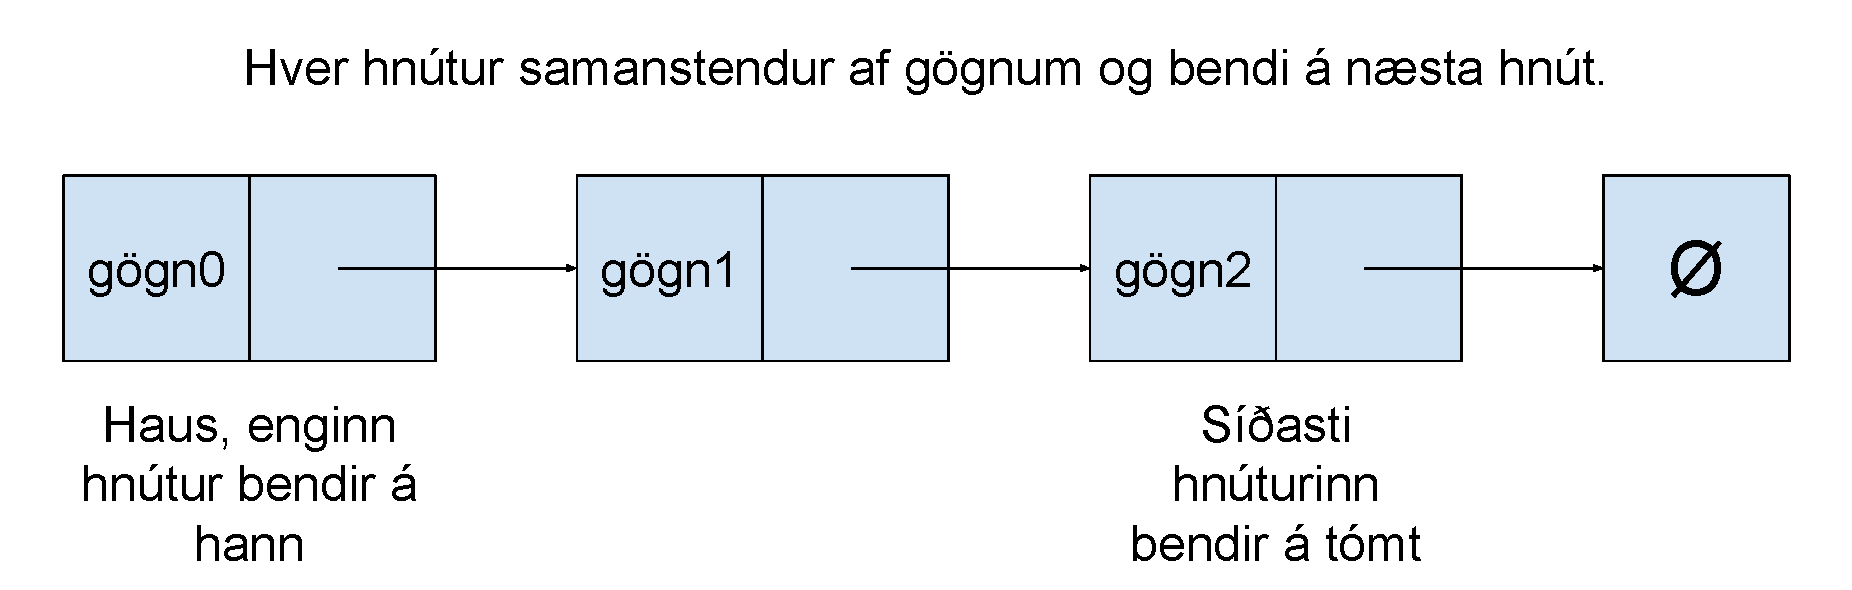
\includegraphics[width=\textwidth]{singly-linked-list}
\end{frame}

\section{Hlutbundin forritun í C++}

\begin{frame}{Hlutbundin forritun}
    \begin{itemize}
        \item Ein aðalástæðan fyrir því að C++ var búið til er að forritunarmálið C styður ekki hlutbundna forritun
        \item Hlutbundin forritun hefur ýmsar birtingarmyndir, en í C++ og málum sem á eftir koma höfum við:
        \begin{itemize}
            \item Hlutir \eng{objects} - grundvallareiningin í hlutbundinni forritun
            \begin{itemize}
                \item Hlutur er ``pakki'' af gögnum og aðgerðum á gögnin
            \end{itemize}
            \item Klasar \eng{classes} eru notaðir til að skilgreina ``gerð'' af hlutum 
        \end{itemize}
        \item Tölum um að hlutur sé tilvik \eng{instance} af klasa
        \item Getum litið á það sem svo að hlutbundin forritun sé leið okkar í C++ til að bæta við tögunarkerfi málsins
    \end{itemize}
\end{frame}

\begin{frame}{Dæmi um klasa}
    Klasi sem táknar mannveru og \texttt{main} fall sem býr til tilvik.
    \begin{columns}
    \column{0.45\textwidth}
        \cppfile[firstline=6, lastline=15, label=human.cpp, fontsize=\tiny, linenos=true]{Code/w2/human.cpp}
    \column{0.45\textwidth}
        \cppfile[firstline=17, lastline=29, label=human.cpp, fontsize=\tiny, linenos=true]{Code/w2/human.cpp}
    \end{columns}
\end{frame}

\begin{frame}{Hlutir og bendar}
    \begin{columns}
        \column{0.45\textwidth}
        \begin{itemize}
            \item Við viljum ekki alltaf vera með hluti á hlaðanum
            \begin{itemize}
                \item Tilvik af klösum geta verið mjög stór, sprengja hlaðann hratt
            \end{itemize} 
            \item Hægt er að vinna með benda á hluti
            \item Til að vísa í eiginleika hlutar út frá bendi er hægt að nota virkjann \texttt{->}
            \item Einnig ekki ómögulegt að sækja fyrst gildið og nota svo punktvirkja
        \end{itemize}
        \column{0.45\textwidth}
        \cppfile[firstline=31, lastline=35, gobble=4, label=human.cpp, fontsize=\tiny, linenos=true]{Code/w2/human.cpp}
    \end{columns}
\end{frame}

\begin{frame}{Smiður og eyðir}
    \begin{itemize}
        \item Gerum ráð fyrir að hugmyndin um smið \eng{constructor} sé þekkt
        \begin{itemize}
            \item Aðferð sem kallað er á þegar tilvik af klasa er búið til
            \item Smiður heitir það sama og klasinn
            \item Ef við skrifum ekki smið fáum við sjálfgefinn smið
        \end{itemize}
        \item í C++ bætum við við hugmyndinni um eyði \eng{destructor} 
        \begin{itemize}
            \item Í eyði eigum við að skila öllum kvikstæðum breytum!
            \item Í C++ heitir eyðir það sama og klasinn, en nú með \textasciitilde{} fyrir framan
            \item Ef við skrifum ekki eyði fáum við sjálfgefinn eyði
        \end{itemize}
    \end{itemize}
\end{frame}

\begin{frame}{Smiður}
    \begin{columns}
    \column{0.45\textwidth}
        \begin{itemize}
            \item Skilgreini forritari smið er sjálfgefna smiðnum ekki bætt við sjálfkrafa
            \item Við getum verið með marga smiði!
            \begin{itemize}
                \item Sjá fjölbindingu, aðeins seinna
            \end{itemize}
            \item Hér sést líka bendirinn \texttt{this}, sem vísar á núverandi tilvik
        \end{itemize}
    \column{0.5\textwidth}
    \cppfile[firstline=6, label=constructhuman.cpp, fontsize=\tiny, linenos=true]{Code/w2/constructhuman.cpp}
    \end{columns}
\end{frame}

\begin{frame}[fragile]{Eyðir}
    \begin{columns}
        \column{0.45\textwidth}
        \begin{itemize}
            \item Líkt og með smiði höfum við líka sjálfgefinn eyði
            \item Ef við úthlutuðum minni með \texttt{new} í klasanum er hér síðasti séns til að gera \texttt{delete}!
            \item ``Þægilegri'' C++ fyrirbrigði eins og \texttt{vector} og \texttt{string} eru með góða eyða
        \end{itemize}
        \column{0.45\textwidth}
        \begin{minted}[frame=lines]{cpp}
class Human {
public:
  ~Human() {
    // destructor code here
  }
};
        \end{minted}
    \end{columns}
\end{frame}

\begin{frame}{Afritun }
    \begin{itemize}
        \item Hlutir sem innihalda benda á kvikstæð minnissvæði geta valdið vandræðum við afritun á hlutum
        \item Ef hluturinn er afritaður, hvað kemur fyrir bendinn?
        \begin{itemize}
            \item Við grunna afritun \eng{shallow copy} er eingöngu bendirinn afritaður 
            \item Við djúpa afritun \eng{deep copy} er afritinu líka úthlutað nýju kvikstæðu minnissvæði
        \end{itemize}
        \item Til að tryggja djúpa afritun í C++ þurfum við að búa til sérstakan afritssmið \eng{copy constructor}
\end{itemize}
\end{frame}

\subsection{Útfærsla á eintengdum lista}

\begin{frame}{Merkilegri klasar}
    \begin{itemize}
        \item Skólabókardæmi um klasa/hluti líkja oft eftir efnislegum hlutum
        \begin{itemize}
            \item Frekar klént
        \end{itemize}
        \item Hlutbundin aðferðafræði er þó iðulega notuð um ``hluti'' sem samsvara ekki neinum hlutum sem hægt væri að snerta
        \begin{itemize}
            \item \texttt{DatabaseConnection}, \texttt{ResourceManager}, \texttt{JSONEncoder}, \ldots
        \end{itemize}
        \item Munum nota hlutbundna forritun til að útfæra ýmsar gagnagrindur
    \end{itemize}
\end{frame}

\begin{frame}[fragile]{Eintengdur listi}
    \begin{columns}
        \column{0.45\textwidth}
        \begin{itemize}
            \item Til hliðar - útfærsla á hnút í eintengdum lista sem geymir heiltölur.
            \begin{itemize}
                \item Við getum lengt listann vandræðalítið
                \item Þurfum að ítra í gegnum listann til að fá aðgang að gögnum
                \item Gögnin eru ekki aðlæg í minni
            \end{itemize}
            \item Allt önnur minnismeðhöndlun en í fylkjum
        \end{itemize} 
        \column{0.55\textwidth}
        \cppfile[label=singlylinked.cpp, linenos=false, firstline=5, lastline=14, fontsize=\small]{Code/w2/singlylinked.cpp}
    \end{columns}
\end{frame}

\begin{frame}{Möguleikar}
    \begin{itemize}
        \item Getum bætt við föllum til að meðhöndla klasann
        \begin{itemize}
            \item Fall til að ná í lengd listans
            \item Fall til að leita að ákveðnum hnút 
            \begin{itemize}
                \item Skila sætisnúmeri eða bendi \pause
            \end{itemize}
            \item Föll til að bæta við gögnum fremst eða aftast \pause
            \item Föll til að bæta við gögnum í ákveðið sæti \pause
            \item Fall til að sækja gögn eftir sætisnúmeri \pause
            \item Fall til að eyða hnúti eftir sætisnúmeri \pause
            \item Fall til að snúa listanum við \pause
        \end{itemize}
        \item Munum kynnast sumum þessara falla!
    \end{itemize}
\end{frame}

\section{Lokaorð}

\begin{frame}{Þessi glærupakki}
    Öll nafngreind forrit í þessum glærupakka, ásamt glærupakkanum sjálfum, má finna á  \href{https://github.com/Ernir/kennsluefni/tree/master/T2/Code/w2}{Github}.
\end{frame}

\begin{frame}{Næst}
Meira um hlutbundna forritun, staðalsafn C++
\end{frame}


\end{document}
